\documentclass{article}
\usepackage[utf8]{inputenc}
\usepackage[T1]{fontenc}
\usepackage{graphicx}
\usepackage{geometry}
\usepackage{float}
\geometry{a4paper, margin=2.5cm}

\title{GRU\_Kod}
\author{Roman}
\date{June 2025}

\begin{document}

\maketitle

\section{Introduction}
To jest wprowadzenie do dokumentu technicznego systemu rekomendacyjnego.

\section{Wizualizacja wyników}

\begin{figure}[H]
\centering
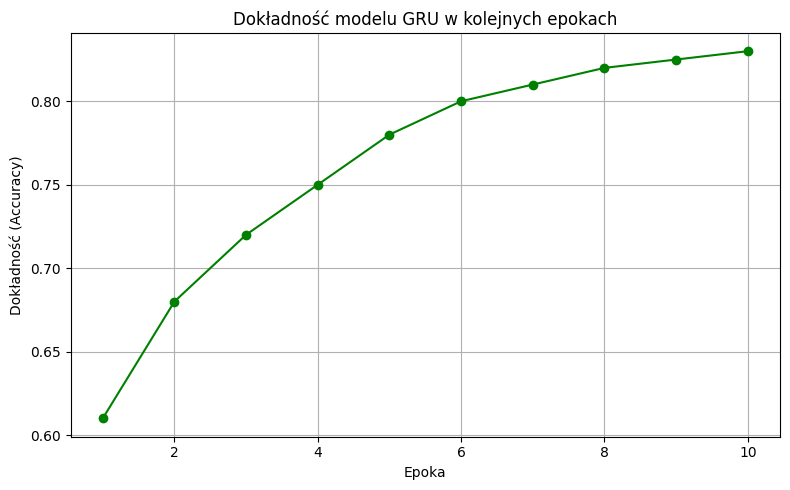
\includegraphics[width=0.8\textwidth]{gru_arch.png}
\caption{Schemat architektury modelu GRU zastosowanego w systemie rekomendacyjnym}
\end{figure}

\begin{figure}[H]
\centering
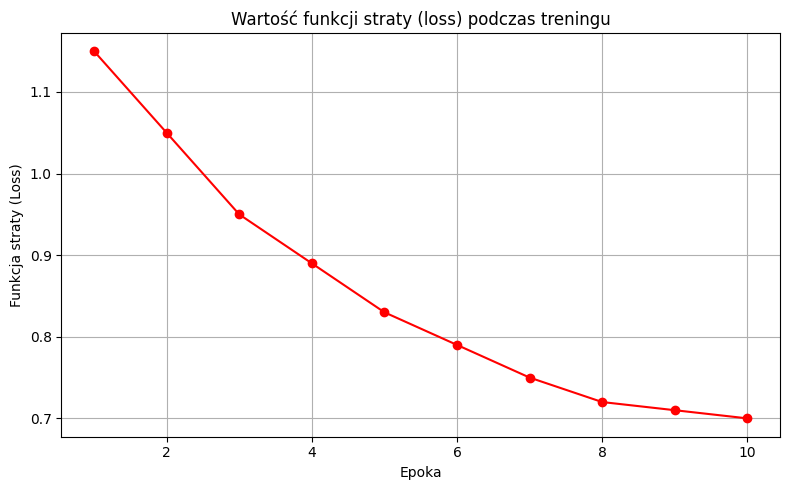
\includegraphics[width=0.8\textwidth]{loss_plot.png}
\caption{Wartość funkcji straty (loss) podczas treningu}
\end{figure}

\begin{figure}[H]
\centering
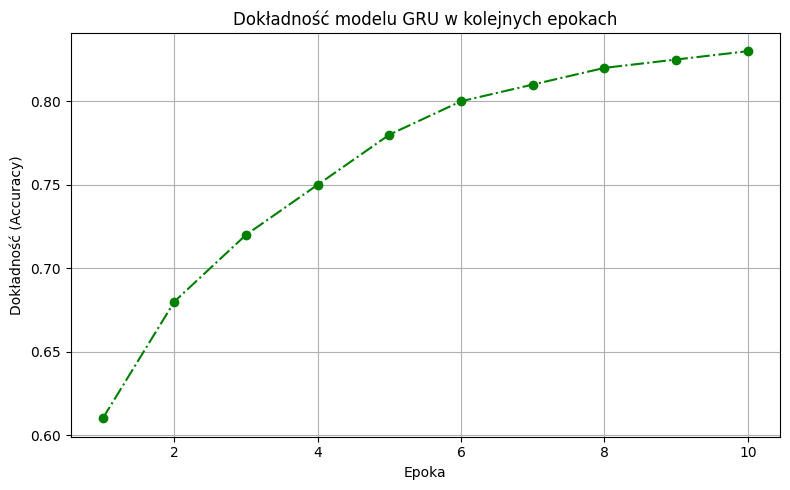
\includegraphics[width=0.8\textwidth]{accuracy_plot.png}
\caption{Dokładność modelu GRU w kolejnych epokach}
\end{figure}

\section{Podsumowanie}
Model GRU został pomyślnie zaimplementowany, a jego wyniki zostały zwizualizowane za pomocą wykresów przedstawionych powyżej.

\end{document}
